\subsection{Somatosensorik \index{Sensorik! Somato-} des Körpers}
Die Somatosensorik des Körpers wird in zwei Systeme unterteilt, wobei der Tastsinn \index{Tastsinn} und die Propriozeption das lemniskale System \index{System! lemniskal} bilden und der Schmerz- und Temperatursinn das anterolaterales System. \index{System! anterolateral} Beide Systeme werden bei Säugern durch die Rezeptoren unter der haarlosen Haut innerviert.

\subsubsection{Tastsinn und Propriozeption (lemniskales System)} \label{subsubsec:tastsinn}

\subsubsection*{Rezeptoren}
Die Rezeptoren \index{Rezeptoren! somatosensorisch} des lemniskalen Systems werden anhand ihrer Lage unter der Haut und ihrer Adaptationseigenschaften unterteilt. Dadurch unterscheiden sie sich in den Modalitäten, die sie kodieren. Bei der Lage wird unterschieden zwischen direkt unter der Oberfläche oder tiefer im Gewebe liegenden Nervenendigungen, sowie schneller bzw. phasischer und langsamer bzw. phasisch-tonischer Adaptation dieser Nerven.\\
Direkt unter der Hautoberfläche liegen die Meissner- und die Merkel-Rezeptoren \index{Rezeptoren! Meissner}\index{Rezeptoren! Merkel}, welche für Bewegung und Druck, sowie in abstrakterem Sinne für Form, Textur und das Greifen nach Objekten kodieren.
\textsuperscript{\cite[Kap.~24]{paxinos2014rat}}. Tiefer unter der Haut liegen die Pacini-Rezeptoren\index{Rezeptoren! Pacini}, welche schnell adaptierende Rezeptoren sind, die für Vibrationen kodieren. Zusammen mit den Meissner- und Merkelrezeptoren bilden sie den bewussten Tastsinn. Die Neurone der Rezeptoren sind dicke, myelinisierte A$\upalpha$ Nervenfasern mit einer Leitgeschwindigkeit von 72-120 m/s \textsuperscript{\cite[Kap.~22]{kandel2013principles}}. Unbewusst werden von den langsamen, tief unter der Haut liegenden, Ruffini-Rezeptoren \index{Rezeptoren! Ruffini} Informationen über die Dehnung der Haut und der Muskeln und damit der Position der Gelenke und Extremitäten, weiter gegeben.
Die Nervenfasern der Propriozeption sind dicke, myelinisierte A$\upbeta$ Nerven, deren Durchmesser etwas geringer ist als der der A$\upalpha$ Neurone.
Die Nervenfasern eines Hautgebiets werden zu einem peripheren Nervenstrang gebündelt und ziehen in das Spinalganglion \index{Spinalganglion} innerhalb des Wirbelkanals. Die Zellkörper der Nervenfasern liegen in diesem Spinalganglion und sind umgeben von speziellen Gliazellen. Zwischen den Nervenzellen verlaufen fenstrierte Kapillaren, die die Nervenfasern mit den nötigen Nährstoffen versorgen. 

\subsubsection*{Rückenmark}
Die Axone der Nerven ziehen weiter ins Rückenmark. Die Axone des lemniskalen Systems ziehen direkt in die weiße Substanz des Rückenmarks und steigen parallel zum Verlauf der Wirbelsäule auf. Die Axone unterhalb des sechsten thorakalen Segments (T6) bilden den \textbf{Fasciculus gracilis} \index{Fasciculus! gracilis} und die Axone oberhalb des sechsten Thorakalsegments (T6) formen den \textbf{Fasciculus cuneatus} \index{Fasciculus! cueatus} im dorsalen Teil der weißen Substanz des Rückenmarks (Abb.~\ref{fig:bahnen_rueckenmark}) \textsuperscript{\cite[Kap.~8]{paxinos2014rat}}. F.~gracilis und F.~cuneatus bilden somit die wichtigste aufsteigende Bahn für die sensorischen Informationen aus dem Tastsinn und der Eigenwahrnehmung hinauf in den Hirnstamm. 
Die Trennung zwischen F.~gracilis und F.~cuneatus ist wichtig, da sie in zwei anatomisch unterschiedlichen Kernen des Hirnstamms terminieren. Sie bilden zusammen mit anderen kleineren Bahnen den Hinterstrang (eng.: dorsal column) \textsuperscript{\cite[Kap.~22]{kandel2013principles}}. 

\begin{figure}[H]
    \centering
    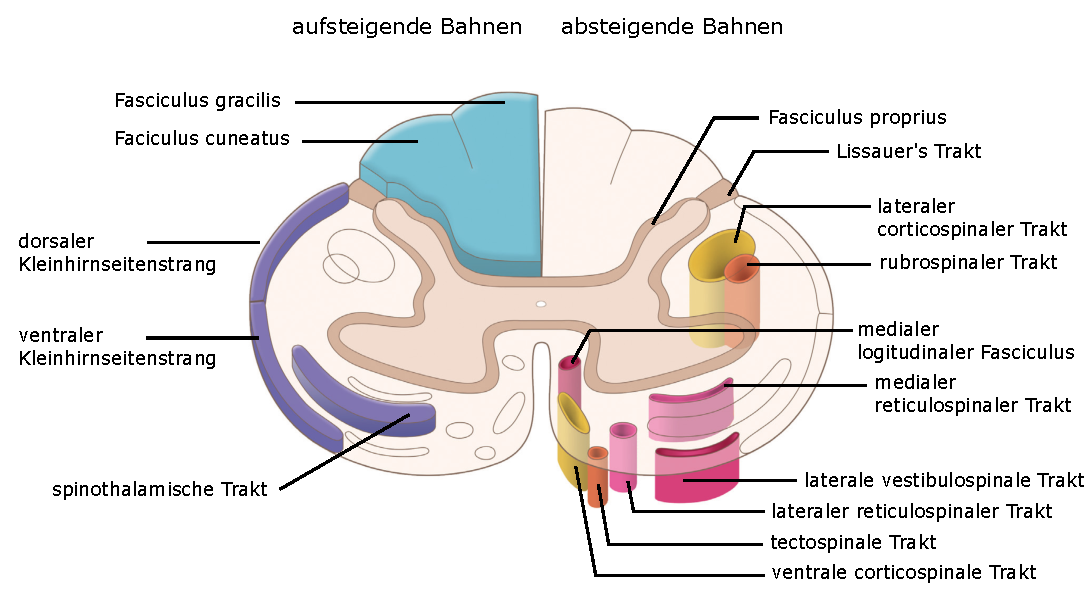
\includegraphics [width = \textwidth]
    {pictures/somatosensory/aufabsteigendeBahnen_Rueckenmark.pdf}
    \caption[Auf- und Absteigende Bahnen im Rückenmark]{\textbf{Auf- und Absteigende Bahnen im Rückenmark.} Zur besseren Veranschaulichung der Bahnen sind die Bahnen in der Abbildung nach absteigenden Bahnen auf der linken Seite und absteigenden Bahnen auf der rechten Seite aufgeteilt. Beide Gruppen kommen jeweils gespiegelt auch auf der anderen Seite vor. \\
    Abbildung aus \textit{Neuroanatomy}, Crossman und Neary
    \textsuperscript{\cite[Kap.~8]{crossman2014neuroanatomy}}.}
    \label{fig:bahnen_rueckenmark}
\end{figure}

\subsubsection*{Nucleus gracilis und Nucleus cuneatus - Medulla}

Die Axone des \textbf{Fasciculus~gracilis} terminieren im \textbf{Nucleus~gracilis} \index{Nucleus! gracilis} in der Medulla. Auf gleicher Ebene der Medulla enden auch die Axone des \textbf{Fasciculus~cuneatus} im \textbf{Nucleus~cuneatus}\index{Nucleus! cuneatus}. Zusammen werden die beiden Kerne auch Hinterstrangkerne\index{Hinterstrangkerne} oder im englischen dorsal column nuclei genannt. In Abbildung~\ref{fig:nucleus_cuneatus} kann man den Nucleus~cuneatus (gelb) sehen. Der Nucleus liegt dorsal des Kerngebiets des Trigeminusnervs (Sp5I) und lateral des vierten Ventrikels (4V). Die Abbildung zeigt nicht den Nucleus gracilis.
\\
\noindent
Beide Nuclei sind zylindrisch geformt und in rostrocaudaler Richtung ausgedehnt. Die afferenten Neurone aus derselben Hautregion enden in der rostrocaudalen Ausdehnung auf einer Linie. Verschiedene Hautregionen werden lateral-medial repräsentiert. Die somatosensorische Repräsentation auf dieser Ebene gleicht einem auf dem Rücken liegenden, kopflosen Homunculus. Dabei liegen die distalen Körperregionen lateral und die proximalen Hautregionen medial in den Nuclei. Die taktilen und propriozeptiven Informationen des Kopfes (Kap.~\ref{sec:somatokopf}) werden in den angrenzenden \textit{Nucleus principalis nervi trigemini} \index{Nucleus! principalis, Pr5} repräsentiert \textsuperscript{\cite[Kap.~22]{kandel2013principles}}. 

\begin{figure}[H]
    \centering
    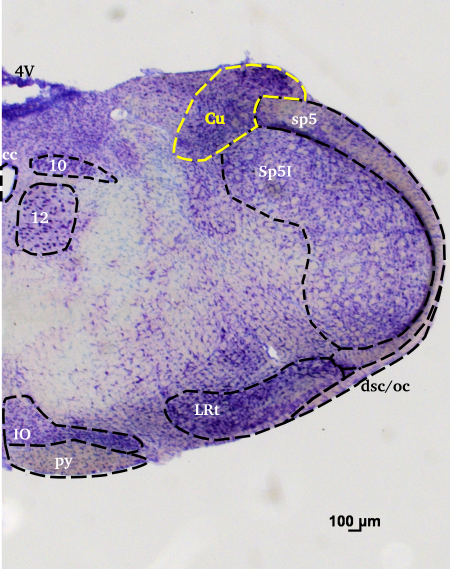
\includegraphics{pictures/somatosensory/nucleus_cuneatus.png}
    \caption[Lage des Nucleus cuneatus in der Medulla]{\textbf{Lage des \textit{Nucleus cuneatus} in der Medulla.} Nissl-Färbung der Rattenhirns auf der Höhe der Medulla (N02-3). Der Ausschnitt zeigt die rechte Seite vom Zentralkanal (cc) bis zum Trigeminusnerv (sp5). Oberhalb des Kerngebiets des Trigeminusnervs (SP5I) liegt der Nucleus~cuneatus (Cu). Die Schnittebene beinhaltet sowohl Teile der Medulla, daran zu erkennen, dass der vierter Ventrikel (4V) angeschnitten ist, als auch Teile des Rückenmarks, daran zu erkennen, dass der Zentralkanal (cc) zu sehen ist. Weitere Kerngebiete sind: der dorsale Kern des Nervus vagus (10), der Kern des Nervus hypoglossus (12), die untere Olive (IO) und der Nucleus reticularis lateralis (LRt). Ebenfalls zu sehen sind die Pyramidenbahn (py), der dorsaler spinocerebellarer Trakt/olivocerebraler Trakt (dsc/oc) und der Trigeminusnerv (sp5).}
    \label{fig:nucleus_cuneatus}
\end{figure}

\subsubsection*{Der Mediale Lemniscus}

\begin{figure}[H]
    \centering
    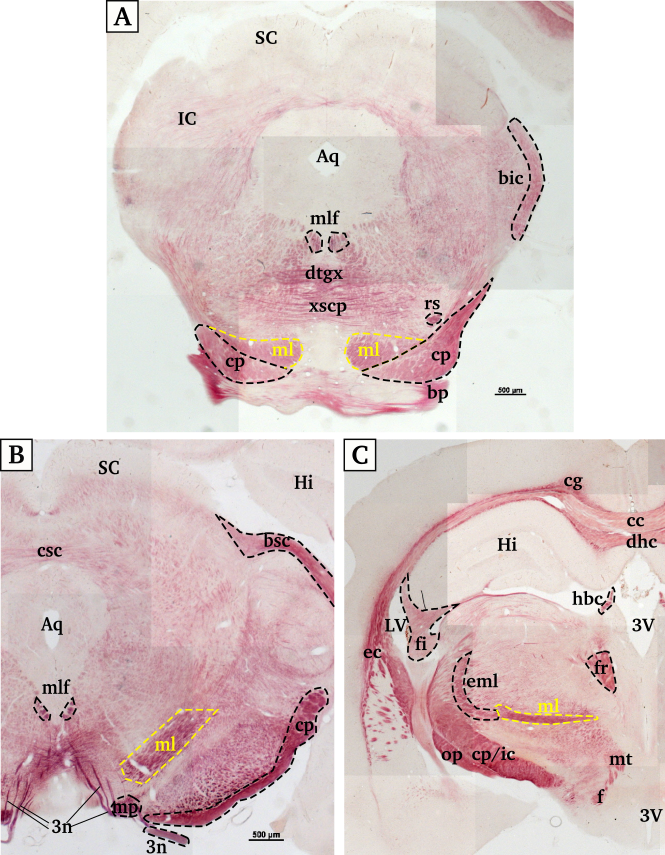
\includegraphics[width = 0.85\textwidth] {pictures/somatosensory/medial_lemniscus.png}
    \caption[Verlauf des medialen Lemniscus]{\small{\textbf{Verlauf des \textit{medialen Lemniscus.}} Faserschnitte auf der Höhe des Mesencephalons (A \& B) und des Diencephalons (C). Man kann den Verlauf des medialen Lemniscus in der Schnittserie über 3450~$\upmu$m verfolgen.\\
    \textbf{A:} (F14-4): Colliculus superior (SC), Colliculus inferior (IC), Aquädukt (Aq), Brachium des IC (bic), brachia pontis (bp, engl.: middle cerebellar peduncle), Großhirnstiele (Pedunculi cerebri) (cp), dorsale tegmentale Dekussation (dtgx), Fasciculus longitudinalis medialis (mlf), rubrospinaler Trakt (rs), Dekussation des SC Pedunkels (xscp).
    \textbf{B:} (F17-3): Nervus oculomotorius (3n), Hippocampus (Hi), Brachium des SC (bsc), Kommissur des SC (csc), Pedunculus mamillaris (mp).
    \textbf{C:} (F20-3): dritter Ventrikel (3V), lateraler Ventrikel (LV), zentrale Kommissur (cc), Cingulum (cg), dorsale Hippocampuskommissur (dhc), Capsula externa (ec), externe medulläre Lamina (eml), Fornix (f), Fimbria (fi), Fasciculus retroflexus (fr), Commissura habenularum (hbc), Capsula interna (ic), mammillothalamischer Trakct (mt), optischer Trakt (op)}}
    \label{fig:medialer_lemniscus}
\end{figure}

In den Hinterstrangkernen ist die erste synaptische Verbindung im lemniskalen System. Von den primär afferenten Axonen aus dem Rückenmark wird das Signal an die Nervenfasern des \textbf{medialen~Lemniscus} \index{Lemniscus! medial} weiter geleitet. Diese kreuzen die Mittellinie auf der Höhe der Medulla und verlaufen anschließend contralateral \textsuperscript{\cite[Kap.~22]{kandel2013principles}}. 
Der \textbf{mediale~Lemniscus} liegt ventral-medial in der Medulla und zieht von der Medulla bis in den Thalamus des Diencephalons. Die Veränderung der Lage des medialen~Lemniscus \index{Lemniscus! medial} kann man in Abbildung~\ref{fig:medialer_lemniscus} verfolgen. Er beginnt bereits auf der Höhe des Nucleus cuneatus (Abb.~\ref{fig:somato_pathway}) und zieht sich dann ventral-medial unterhalb des Aquädukts (Abb.~\ref{fig:medialer_lemniscus}~A) weiter in rostraler Richtung. Dabei verändert er seine Lage in sofern, dass er von ventral-medial nach medial-lateral (Abb.~\ref{fig:medialer_lemniscus}~B) zieht. Der mediale~Lemniscus zieht auf der Höhe des dritten Ventrikels (Abb.~\ref{fig:medialer_lemniscus}~C) zentral im Diencephalon bis in den Thalamus.

\subsubsection*{Thalamus im lemniskalen System}
\index{Thalamus! lemniskales System}
Die Informationen aus den Hautschichten von den Meissner-, Merkel- und Pacini-Rezep-toren, die über die primär afferenten Neurone und den medialen Lemniscus kommen, werden im lateralen und medialen \textbf{Nucleus ventralis posterior} (eng.: lateral and medial
ventral posterior nuclei) \index{Nucleus! ventralis posterior} verarbeitet. Propriozeptive Informationen aus den Gelenken und dem Bauchraum werden über den medialen Lemniscus an den oberen Nucleus ventralis posterior (eng.: superior ventral posterior nucleus) weitergeleitet \textsuperscript{\cite[Kap.~22]{kandel2013principles}}. 
In der Nisslfärbung des Rattenhirns ist keine Abgrenzung der einzelnen Nuclei des Thalamus sichtbar. Der Thalamus, als Verschaltungszentrale des Diencephalons, liegt bei der Ratte zentral über, bzw. lateral des dritten Ventrikels (3V, Abb.~\ref{fig:thalamus_somato}) und oberhalb des Hypothalamus. 
Am Beispiel des Menschen werden in Kapitel \label{subsubsec:thalamus} die einzelnen Kerne im Thalamus gezeigt, wobei die Lage der somatosensorischen Kerne gut in Abbildung \ref{fig:thalamus_nuclei}~A~\&~B zu sehen ist.
Die zweite synaptische Verschaltung im Thalamus gibt die Informationen an die Neurone der thalamisch-cortikalen Verbindung weiter, welche die Informationen dann an den primären somatosensorischen Cortex leitet.

\begin{figure}[H]
    \centering
    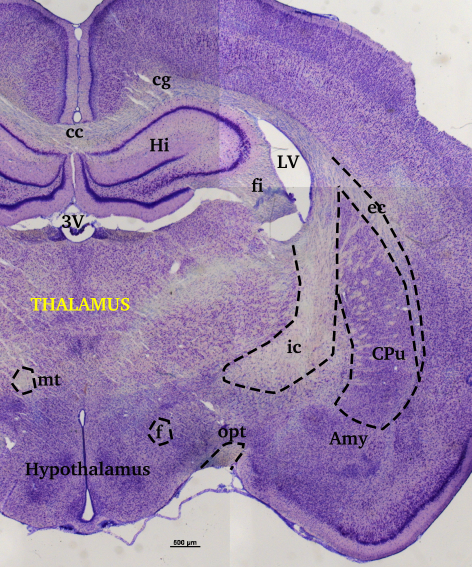
\includegraphics[width = 0.8\textwidth]
    {pictures/somatosensory/thalamus_somato.png}
    \caption[Thalamus im lemniskalen System]{\textbf{Thalamus im lemniskalen System.} Rechte Gehirnhälfte (N23-3) der Ratte auf der Höhe des Thalamus und des dritten Ventrikels (3V). Auf derselben Höhe sind als prominente Hirnstrukturen der Hippocampus (Hi), der Hypothalamus und die zentrale Kommissur (Corpus callosum, cc) zu sehen. Weitere Strukturen sind Cortex, Amygdala (Amy), Caudate Putamen (CPu), Cingulum (cg), äußere Kapsel (ec), Fornix (f), Fimbria (fi), innere Kapsel (ic), lateraler Ventrikel (LV), mammillothalamischer Trakt (mt), optische Bahn (opt).}
    \label{fig:thalamus_somato}
\end{figure}

\subsubsection*{Primärer Somatosensorischer Cortex}
\label{subsubsec:S1}
Der \textbf{somatosensorische Cortex} \index{Cortex! primär somatosensorisch} liegt beim Menschen auf dem postzentralen Gyrus,\index{Gyrus! postzentral} direkt hinter dem \textit{Sulcus centralis}. Der primäre somatosensorische Cortex (S1) setzt sich aus den Brodmann-Arealen 3a, 3b, 1 und 2 zusammen und endet anterior im Sulcus centralis, wo er an den primären Motorcortex (Brodmann-Areal~4) angrenzt. Posterior des S1 liegt der posteriore Parietallappen mit den Brodmann-Arealen 5 und 7. In Abbildung~\ref{fig:S1_Cortex} ist ein horizontaler Schnitt durch die verschiedenen Areale des primären somatosensorischen Cortex und den angrenzenden Strukturen zu sehen \textsuperscript{\cite[Kap.~23]{kandel2013principles}}. 

\begin{figure}[H]
    \centering
    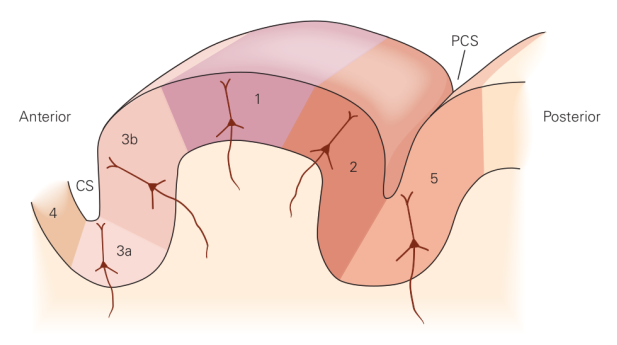
\includegraphics{pictures/somatosensory/S1_Cortex.png}
    \caption[Primärer somatosensorischer Cortex]{\textbf{Primärer somatosensorischer Cortex (S1).} Der primäre somatosensorische Cortex (S1) setzt sich aus den Brodmann-Arealen 3a, 3b, 1 und 2 zusammen und endet anterior im Sulcus centralis (CS). Dort grenzt er an den primären Motorcortex (Brodmann-Areal 4). Posterior des S1 liegt der posteriore Parietalcortex mit den Brodmann-Arealen 5 und 7. Er grenzt sich vom postzentralen Gyrus durch den postzentralen Sulcus (PCS) ab. Abbildung aus \textit{Principles of Neural Systems}, Kandel et al. \textsuperscript{\cite[Kap.~23]{kandel2013principles}}.}
    \label{fig:S1_Cortex}
\end{figure}

Betrachtet man den somatosensorischen Cortex in seiner Ausdehnung entlang des Sulcus centralis \index{Sulcus! centralis}, wie auch die Schnittebene in Abbildung~\ref{fig:somato_pathway} verläuft, wird nochmal die Somatotopie \index{Somatotopie} deutlich. Hierbei ist vor allem der Unterschied zwischen den Tieren sehr prominent. Die somatosensorischen Informationen auf der Hautoberfläche unterscheiden sich in der Größe der rezeptiven Felder und in der daraus resultierenden Relevanz. Auf Grund dessen werden einige Körperregionen mehr repräsentiert als andere. Eine Darstellung dieser Überrepräsentation ist der Homunculus (Abb.~\ref{fig:somato_homunculus}). Der Homunculus \index{Homunculus} der Ratte ähnelt dem des Kaninchens.


\begin{figure}[H]
    \centering
    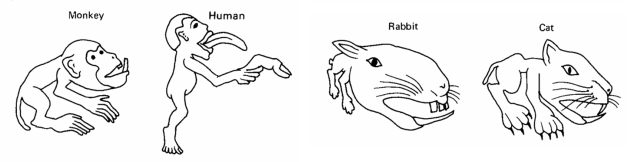
\includegraphics[width = \textwidth] {pictures/somatosensory/homunculus.png}
    \caption[Homunculus]{\textbf{Homunculus.} Homunculi des Affen, Menschen, Kaninchens und der Katze. Abbildung aus der Vorlesung \textit{Integrative Neurobiology: Somatosensory System}, J. Ostwald \textsuperscript{\cite{Ostwald}}.}
    \label{fig:somato_homunculus}
\end{figure}

\newpage
Areal~3b erhält Informationen aus den bewussten Mechanorezeptoren der Haut. In diesem Cortexareal werden vor allem die Wahrnehmung der taktilen Reize und deren Form und Textur verarbeitet, wohingegen in Areal~3a die Wahrnehmung aus der Körperhaltung und der Propriozeption verarbeitet wird. Areal~1 und 2 erhalten ihre Informationen aus Areal~3b. In Areal~1 werden die Informationen aus der strukturellen Beschaffenheit des Objekts weiterverarbeitet, in Areal~2 Informationen über die Größe und Gestalt. Alle vier Areale des primären somatosensorischen Cortex projizieren in den sekundären somatosensorischen Cortex (S2) \textsuperscript{\cite[Kap.~12]{neurowissenschaften_baer}}.
\\
\noindent Der sekundäre somatosensorische Cortex \index{Cortex! sekundär somatosensorisch} liegt unterhalb des primären somatosensorischen Cortex und ist für die Verarbeitung der Informationen aus beiden S1 zuständig. Über den Corpus callosum erhält er Informationen aus der jeweils anderen Großhirnhemispäre. Er verarbeitet die bilateralen rezeptiven Felder und ist für den Lerntransfer zwischen den beiden Hemispären zuständig. Der S2 ist auch für die generelle Aufmerksamkeit bezüglich taktiler Informationen verantwortlich \textsuperscript{\cite[Kap.~12]{neurowissenschaften_baer}}.

Im Gegensatz zu der Lage des somatosensorischen Cortex beim Menschen steht die Lage bei der Ratte. Da Ratten ein lisencephales Gehirn besitzen und bei diesen Tieren kein Sulcus centralis ausgebildet ist, ist die Lokalisation des Areals nicht anhand dessen zu bestimmen. Anhand der Schichtung und Färbungen wurde der somatosensorische Cortex bei der Ratte identifiziert (Abb.~\ref{fig:S1_Cortex_Ratte}). Die Neurone in dem Teil des Cortex (anteriore parietale Region) wurden durch eine stark ausgeprägte granuläre Schicht IV und der stärksten Myelinisierung aller Cortexareale identifiziert. \textsuperscript{\cite[Kap.~22]{paxinos2014rat}}
\\
\begin{figure}[H]
    \centering
    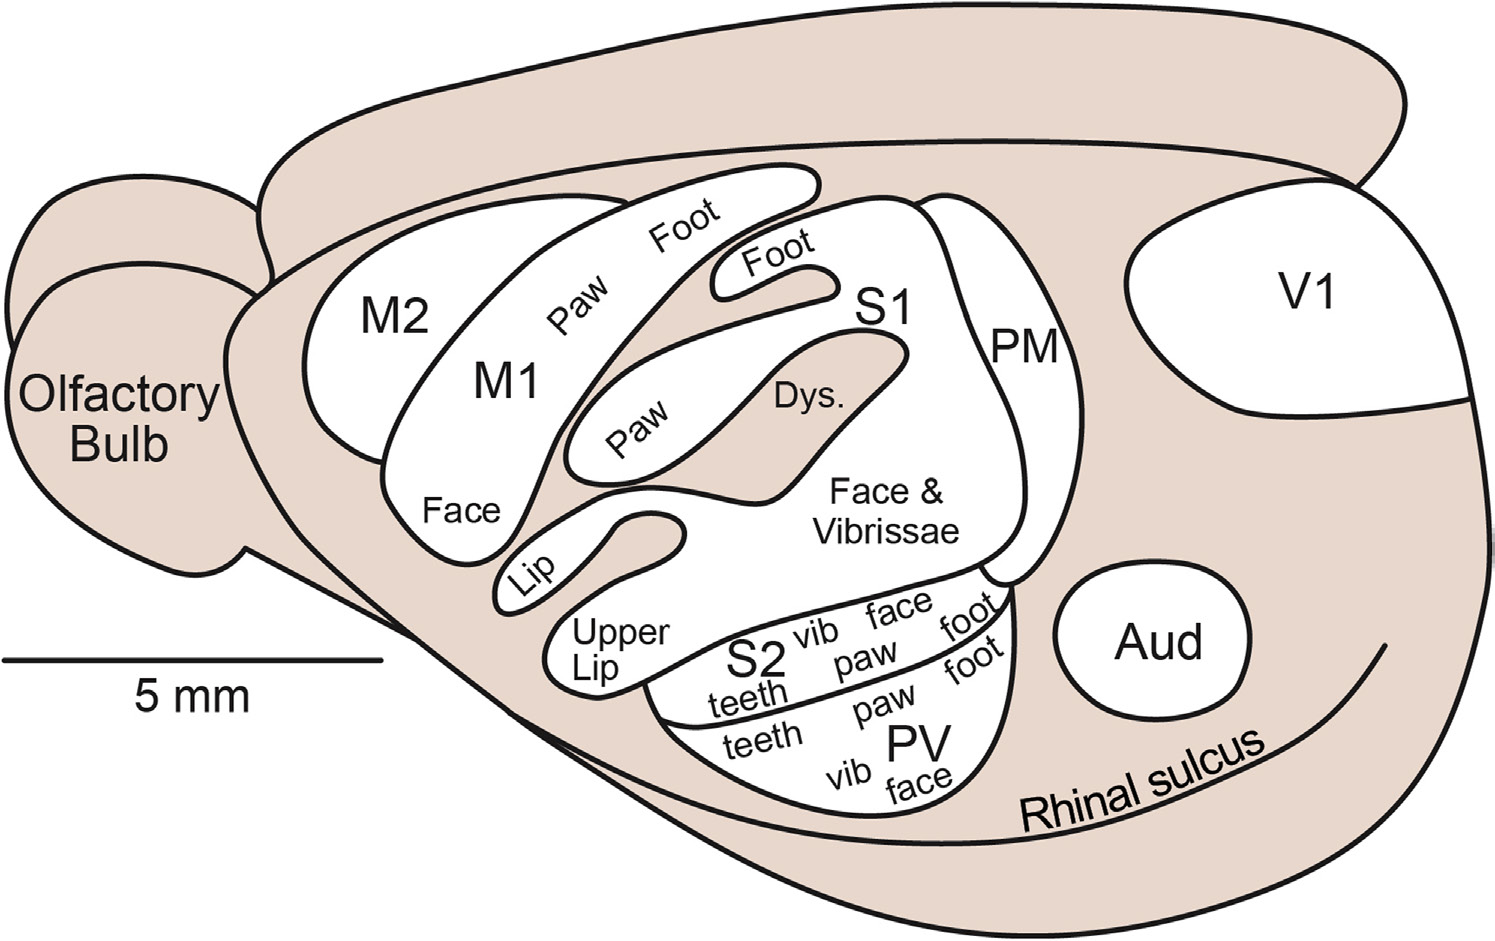
\includegraphics[width = 0.8\textwidth] {pictures/somatosensory/Somato_cortex_ratte.png}
    \caption[Somatosensorischer Cortex der Ratte]{\textbf{Somatosensorischer Cortex der Ratte.} Primärer (S1) und sekundärer (S2) somatosensorischer Cortex mit der Repräsentation der einzelnen Körperregionen. Außerdem ist die \textit{Fissura rhinalis} (Rhinal sulcus) gezeigt, welche den Neocortex vom Archicortex trennt. Anterior vom somatosensorischen Cortex ist der Motorcortex mit primärem (M1) und sekundärem (M2) Motorcortex. Ventral des S2 liegt das parietale ventrale somatosensorische Areal (PV) und posterior das posteriore mediale Areal (PM). Als Reverenz sind noch der auditorische Cortex (Aud) und der visuelle Cortex (V1) gezeigt. Abbildung aus \textit{The Rat Nervous System}, Paxinos et al. \textsuperscript{\cite[Kap.~24]{paxinos2014rat}}.}
    \label{fig:S1_Cortex_Ratte}
\end{figure}

\subsubsection*{Somatosensorische Bahnen}

\begin{figure}[H]
    \centering
    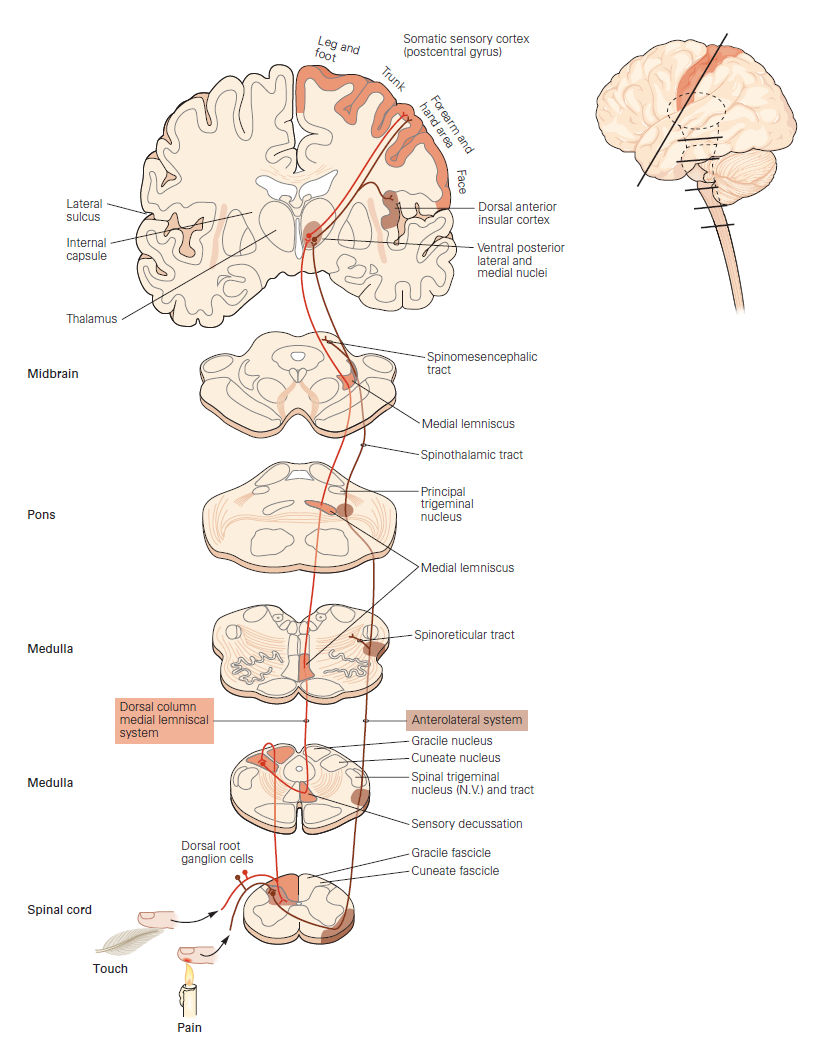
\includegraphics{pictures/somatosensory/pathway_somatosensory2.png}
    \caption[Aufsteigende Bahnen der Somatosensorik]{\textbf{Aufsteigende Bahnen der Somatosensorik.} Die aufsteigenden Bahnen der Somatosensorik sind getrennt in das lemniskale (rot) und das anterolaterale (braun) System. Beginnend im Rückenmark bis hin zum primären somatosensorischen Cortex posterior vom \textit{Sulcus centralis}. Die Bahnen sind am Beispiel des Menschen schematisch dargestellt und sind auf den Ebenen des Rückenmarks, der Medulla, der Pons, des Mittelhirns und des Cortex zu verfolgen.\\
    Abbildung aus \textit{Principles of Neural Science}, Kandel et al. \textsuperscript{\cite[Kap.~22]{kandel2013principles}}.}
    \label{fig:somato_pathway}
\end{figure}

\newpage    
\subsubsection{Schmerz und Temperatursinn (anterolaterales System)}
\label{subsubsec:Schmerzsinn}
\index{System! anterolateral}
Der Schmerz- und Temperatursinn \index{Schmerzsinn} \index{Temperatursinn} hat vor allem eine schützende Funktion auf unseren Körper. Er wird unter dem Begriff der Nozizeption (lat.: 'nocere' für Schaden) zusammengefasst. Er warnt uns vor Verletzungen oder zu großer Hitze, worauf wir dann reflexartig reagieren und zurückweichen oder die Verletzung behandeln können. Die Schmerzwahrnehmung geht von den somatosensorischen Strukturen in der Haut aus und wird von dort zu den höheren Gehirnarealen weitergeleitet.

\subsubsection*{Rückenmark}

Die meisten der Nozizeptoren \index{Nozizeptoren} sind einfache Nervenendigungen primärer sensorischer Faser und können generell in drei Gruppen eingeteilt werden, die thermischen, mechanischen und polymodalen Nozizeptoren \textsuperscript{\cite[Kap.~24]{kandel2013principles}}. Auch die Zellkörper der Nozizeptoren des Körpers liegen im dorsalen Wurzelganglion und terminieren im Hinterhorn des jeweiligen Segments. Ihre Synapsen konzentrieren sich in den Schichten I, IV, V, VII, und X des Hinterhorns (Abb.~\ref{fig:graymatter}) \textsuperscript{\cite[Kap.~25]{paxinos2014rat}}.

\begin{figure}[H]
        \centering
        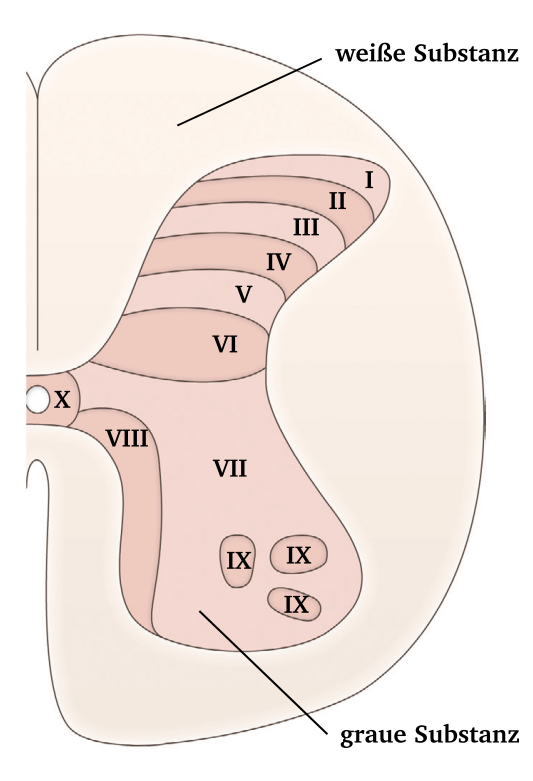
\includegraphics[width = 0.5\textwidth]
        {pictures/somatosensory/gray_matter.png}
        \caption[Schichten in der grauen Substanz des Rückenmarks]{\textbf{Schichten in der grauen Substanz des Rückenmarks.} Die Abbildung zeigt schematisch die rechte Seite des Rückenmarks mit weißer und grauer Substanz. Die Schichten der grauen Substanz beginnen im Hinterhorn mit Schicht I und gehen bis Schicht VIII im Vorderhirn. Die Schicht XI liegt in Schicht VIII. Schicht X umgibt den Zentralkanal. Abbildung nach \textit{Neuroanatomy}, Crossman und Neary
        \textsuperscript{\cite[Kap.~8]{crossman2014neuroanatomy}}.}
        \label{fig:graymatter}
    \end{figure}

\newpage
Diese Synapsen verbindet die Nozizeptoren mit den spinothalamischen Neuronen. Wie der Name dieser Neurone bereits sagt, ziehen sie vom Rückenmark bis in den Thalamus. Die Zellkörper der Neurone liegen in der grauen Substanz des Rückenmarks, während die Axone in der weißen Substanz des Rückenmarks parallel zum Verlauf der Wirbelsäule in Bahnen auf- und absteigen. Die Axone der spinothalamischen Nervenzellen kreuzen auf der Ebene der ersten Synapse die Mittellinie und steigen in der contralateralen weißen Substanz zum lateralen Bereich des Thalamus auf. Bei Ratten bildet die größte Gruppe der spinothalamischen Neurone, jene, welche auf der Höhe der Halswirbelsäule der grauen Substanz beginnen \textsuperscript{\cite[Kap.~25]{paxinos2014rat}}.


\subsubsection*{Thalamus im anterolateralen System}
\index{Thalamus! anterolaterales System}
Die aufsteigende spinothalamische Bahn \index{Tractus! spinothalamisch} im Rückenmark ist anhand ihrer Verbindung von Rückenmark und Thalamus benannt und verläuft ventral des Vorderhorns \index{Vorderhorn} (Abb.~\ref{fig:bahnen_rueckenmark}). Auch diese Neurone sind somatotop organisiert. Die Axone aus Schicht I steigen im lateralen Funiculus,\index{Funiculus! lateral} auf, wohingegen die Axone aus den Schichten IV, V und X in der ventralen weißen Substanz aufsteigen und in den medialen und intralaminaren Thalamus projizieren \textsuperscript{\cite[Kap.~25]{paxinos2014rat}}. 
Mehrere Nuclei des Thalamus verarbeiten die Informationen aus dem anterolateralen Sytem. Die wichtigsten zwei Gebiete sind die lateralen und die medialen Kerngebiete. 
Die lateralen Kerngebiete bestehen aus dem ventro-posterior medialen Nucleus, dem ventro-posterior lateralen Nucleus und dem posterioren Nucleus. Sie erhalten Informationen über Nozizeption-spezifische Neurone mit breitem dynamischen Spektrum. Dieses Kerngebiet beschäftigt sich deshalb unter anderem mit der präzisen Lokalisation von Verletzungen und der Übertragung dieser Informationen als bewussten Schmerz \textsuperscript{\cite[Kap.~24]{kandel2013principles}}.
\\
\noindent Die medialen Kerngebiete des Thalamus setzen sich aus dem zentral-lateralen Nucleus und dem intralaminaren Komplex zusammen. Sie bekommen unter anderem Input aus dem spinothalamischen Trakt, aber auch aus der \textbf{Formatio reticularis}.\index{Formatio reticularis} Neurone im medialen Thalamus reagieren auf schädigende Stimuli und projizieren in die Basalganglia und den Cortex \textsuperscript{\cite[Kap.~24]{kandel2013principles}}.

\subsubsection*{Cortex}
\index{Cortex! somatosensorisch}
Bei \textbf{Ratten} wurden Reaktionen auf einen schädigenden Stimulus im primären somatosensorischen Cortex festgestellt. Demnach werden hier zum Teil die Informationen aus dem anterolateralen System verarbeitet. Die Neurone aus dem nozizeptiven System befinden sich in der Schicht V und VI des somatosensorischen Cortex, wohingegen sich die mechanorezeptiven Neurone in Schicht II~-~V befinden. Die rezeptiven Felder des Schmerz- und Temperatursinns im Cortex sind im Vergleich zu den der mechanosensorischen rezeptiven Felder größer und zudem meist inhibitorisch \textsuperscript{\cite[Kap.~25]{paxinos2014rat}}.
\\
\noindent Im Gegensatz dazu steht die Verarbeitung der Schmerz- und  Temperaturwahrnehmung beim \textbf{Menschen}. Einige der Neurone im \textit{Gyrus cinguli},\index{Gyrus! cinguli} oberhalb des \textit{Corpus callosum},\index{Corpus! callosum} und der Inselrinde (\textit{Cortex insularis}),\index{Insula} innerhalb des Sulcus lateralis, reagieren stark und ausschließlich auf Reize aus dem nozizeptiven somatosensorischen System. Der Gyrus cinguli ist wie schon in Kapitel \ref{subsubsec:Grosshirnrinde} und \ref{subsec:limisches_system}) beschrieben, ein Teil des limbischen Systems. Es wird vermutet, dass das limbische System bei der Verarbeitung von Gefühlszuständen, assoziiert mit der Schmerzwahrmnehmung, beteiligt ist. Neurone des Thalamus projizieren direkt zur Inselrinde (Insula)\index{Insula}, vor allem aus dem medialen und venteroposterior-medialen Nucleus des Thalamus. Die Inselrinde verarbeitet hauptsächlich Informationen über den Zustand innerhalb des Körpers und wirkt bei der autonomen Reaktion des Körpers auf den Schmerz mit \textsuperscript{\cite[Kap.~24]{kandel2013principles}}.

\subsubsection*{Spinomesencephalischer Trakt und  Spinoreticularer Trakt}

Sowohl der spinomesencephalische Trakt\index{Tractus! spinomesencephal}, als auch der spinoreticuläre Trakt\index{Tractus! spinoreticulär} sind Abzweigungen vom spinothalamischen Trakt. Es ist bekannt, dass der spinoreticuläre Trakt bei der absteigenden Schmerzunempfindlichkeit und bei autonomen Regulationen eine Rolle spielt. Der spinomesencephalische Trakt ist an der Schmerzwahrnehmung beteiligt. Dabei ist er für den motivational-affectiven Aspekt, also für die Vermeidung von Schmerz, weil er unangenehm ist, zuständig. Aus diesem Grund ist der spinomesencephalische Trakt auch beim Auslösen von Aktivität im absteigenden Kontrollsystem involviert \textsuperscript{\cite[Kap.~24]{kandel2013principles}}.


